\chapter{METODOLOGI}

\section{Metode yang digunakan}

Penelitian ini dilaksanakan sesuai dengan blok diagram pada Gambar 3.1. Blok diagram tersebut
merupakan metodologi penelitian yang disusun sesuai dengan langkah-langkah yang dilakukan dalam penelitian ini.

\begin{figure} [ht] \centering
  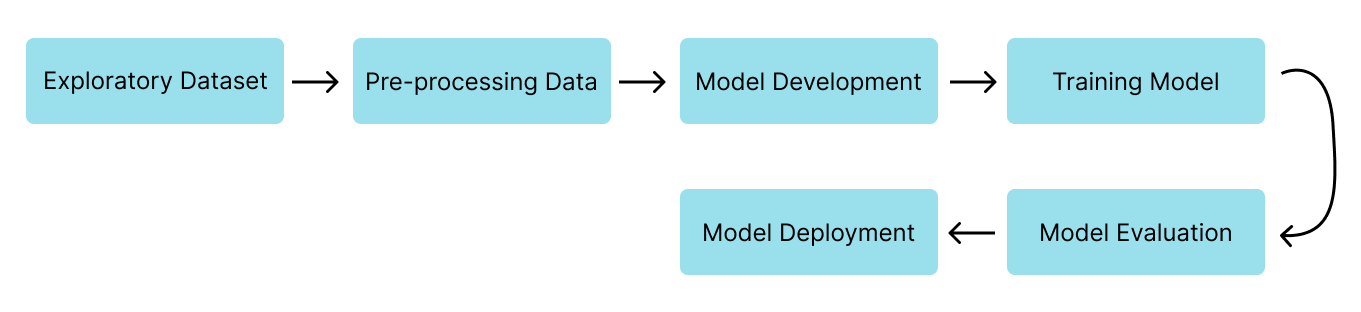
\includegraphics[width=160mm]{gambar/diagram-blok.png}
  \caption{Metodologi Penelitian}
\end{figure}

\section{Bahan dan peralatan yang digunakan}
\begin{enumerate}
  \item Komputer/Laptop
  \item Python
  \item Jupyter Notebook
  \item Tensorflow
  \item Docker
  \item Flask
\end{enumerate}

\section{Urutan pelaksanaan penelitian}

\begin{adjustwidth}{1em}{0pt}
  \addtocontents{toc}{\protect\setcounter{tocdepth}{1}}

  \subsection{Explorasi Dataset}
  Melakukan analisa pada data untuk mendapatkan gambaran awal pada data. Analisa yang dilakukan yaitu
  memeriksa informasi pada data (tipe data pada tiap data), memeriksa \emph{missing value} {(data yang hilang pada baris data)},
  memeriksa duplikasi pada data.

  \subsection{Pre-pemrosesan Data}
  Pada proses ini dataset yang telah dilakukan analisa akan dilakukan pra-pemrosesan sebelum dataset dapat digunakan
  untuk melakukan pelatihan pada model. Pada sistem rekomendasi pra-pemrosesan data yang biasa dilakukan seperti menghapus data
  yang tidak diperlukan untuk proses pelatihan, menghapus \emph{missing value} jika ada, melakukan normalisasi pada data (biasanya mentransformasikan data kedalam range yang sama),
  melakukan pembagian data pelatihan dan data percobaan.

  \subsection{\emph{Grades Prediction}}
  Untuk dapat menemukan mata kuliah yang mungkin sesuai dengan minat mahasiswa, diperlukan model yang dapat memprediksi nilai mata kuliah yang kemungkinan akan diambil oleh mahasiswa. Ini
  merupakan salah satu tahap dalam membangun sistem rekomendasi dengan pendekatan \emph{collaborative filtering} yang mana model akan memprediksi nilai yang akan didapatkan oleh mahasiswa dari berbagai mata kuliah
  yang belum pernah diambil sebelumnya oleh mahasiswa. Nilai yang diprediksi tidak hanya berdasarkan dari riwayat pengambilan mata kuliah dari satu orang mahasiswa, namun akan dilakukan pencocokan dengan mahasiwa
  lain yang memiliki preferensi yang saama. Setelah memprediksi nilai dari sekumpulan mata kuliah nantinya akan diambil \emph{top-N} mata kuliah dengan prediksi nilai tertinggi, setelah itu mata kuliah tersebut dapat direkomendasikan
  kepada mahasiswa.

  \subsection{\emph{Similarity Measure}}
  Tahap ini merupakan penerapan untuk pendekatan \emph{content-based filtering} yang mana model akan mencari kemiripan dari suatu mata kuliah, berdasarkan karakteristik yang dimiliki oleh mata kuliah tersebut.
  Setelah mendapatkan mendapatkan daftar mata kuliah yang mirip dengan input mata kuliah yang diberikan, hasil tersebut akan dikombinasikan dengan hasil rekomendasi dari model dengan pendekatan \emph{collaborative filtering}
  sehingga menghasilkan sistem rekomendasi dengan pendekatan \emph{hybrid recommender syste}.

  \subsection{Evaluasi Model}
  Evaluasi Model dilakukan dengan melakukan rekomendasi pada data percobaan. Jika dirasa rekomendasi belum cukup baik. Maka perlu melakukan \emph{tuning parameter} pada model seperti unit layer,
  jumlah layer pada model \emph{Deep Learning}, jumlah iterasi pelatihan dan beberapa parameter lain hingga model dapat memberikan rekomendasi dengan cukup baik.

  \subsection{\emph{Retrieval Recommendations}}
  Pada tahap ini model dari sistem rekomendasi yang telah dibuat sebelumnya ada dideploy atau dirilis agar dapat digunakan untuk memberikan rekomendasi melalui sebuah \emph{software}.
  \emph{Software} yang digunakan untuk menampilkan rekomendasi dari mata kuliah yang diberikan oleh model tersebut berupa website sederhana yang bisa menampilkan daftar mata kuliah
  yang direkomendasikan sesuai dengan ID/NRP dari mahasiswa.

  \begin{figure} [ht] \centering
    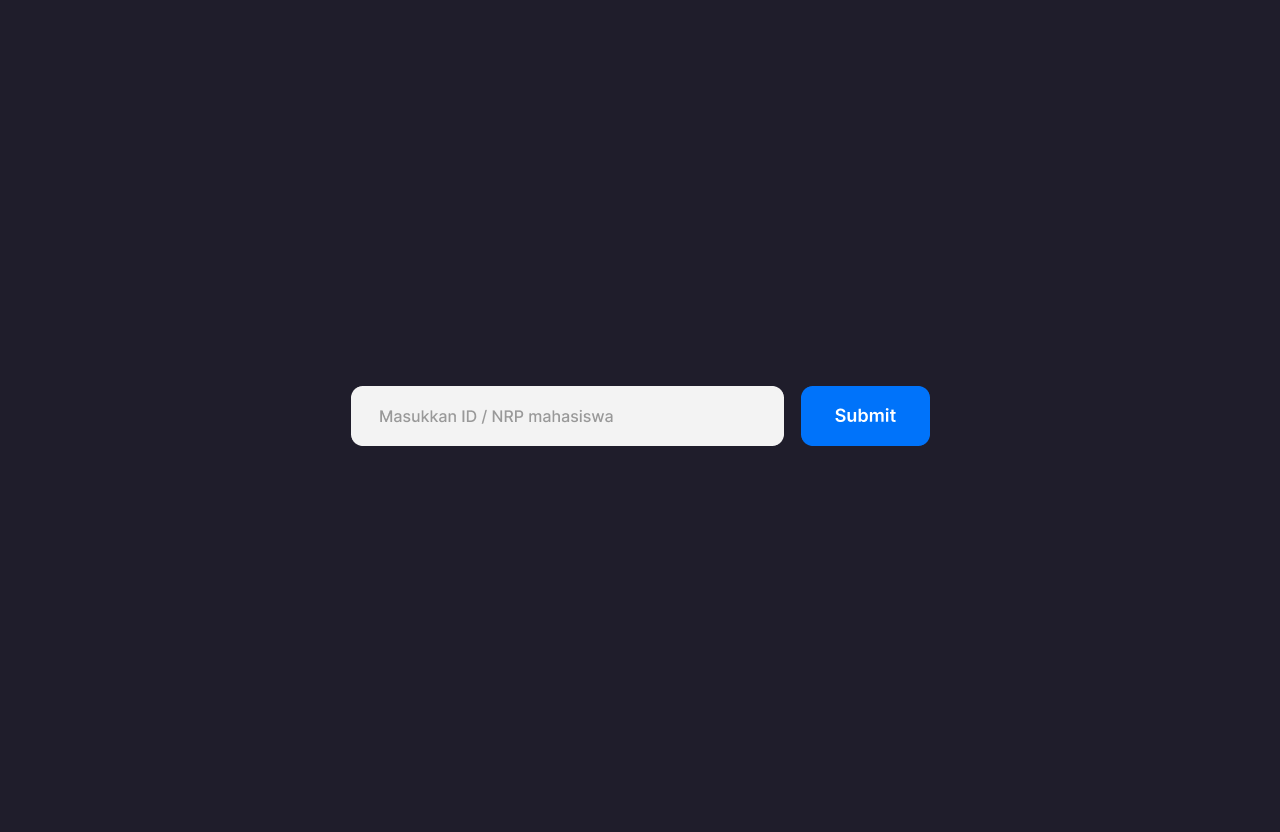
\includegraphics[width=150mm]{gambar/mockup-1.png}
    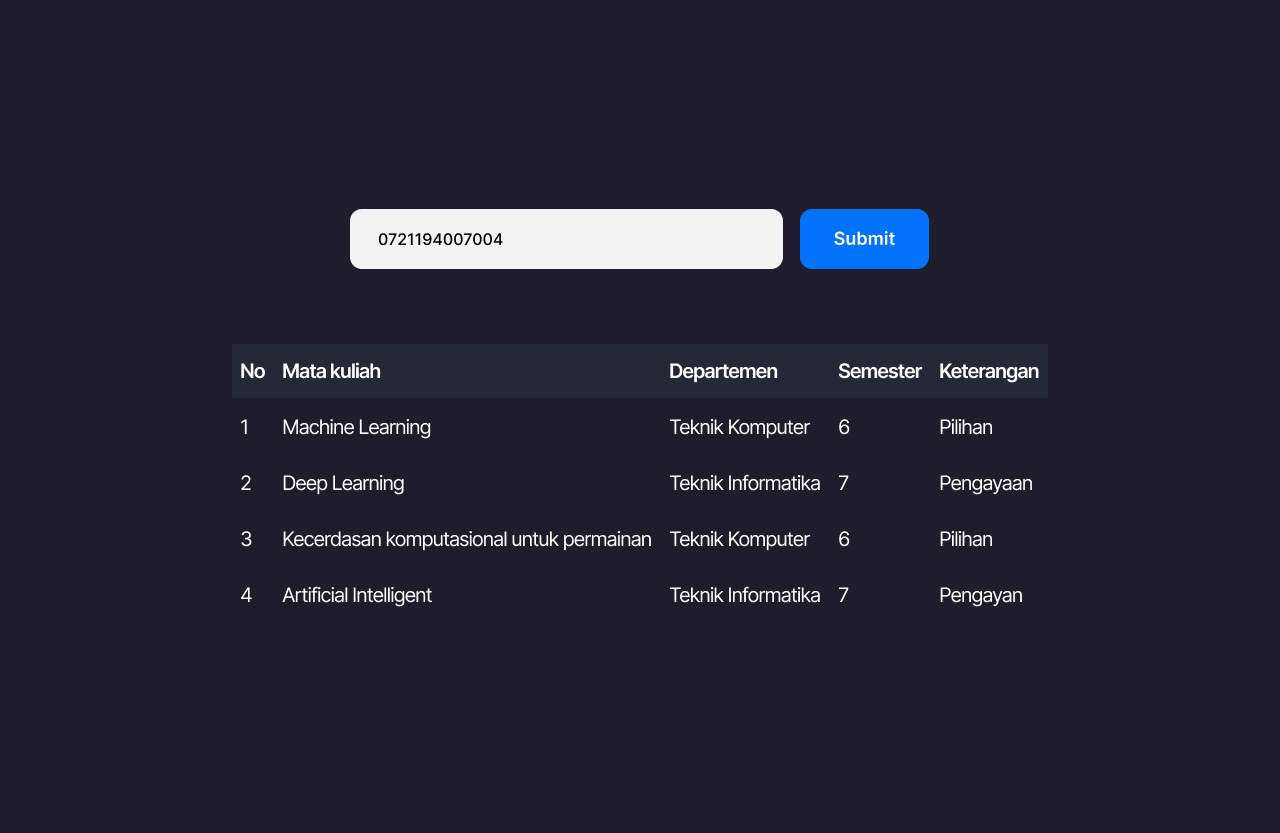
\includegraphics[width=150mm]{gambar/mockup-2.png}
    \caption{Mock Up Tampilan Website Sederhana}
  \end{figure}

\end{adjustwidth}



